\section{各画面の説明}
\subsection{ログイン画面}
\subsubsection{画面の概要}
% 画面の概要
この画面は、システムを利用する管理者および学生がログインするためのものです。
図\ref{fig:01}、\ref{fig:02}にイメージ図を示します。

\subsubsection{操作説明}
% 操作説明
ログインする場合は、ユーザIDとパスワードを入力し、「ログイン」ボタンを押します。
ログインが成功すると、管理者アカウントの場合は「管理者用ホーム画面」に遷移し、
学生アカウントの場合は「学生用ホーム画面」に遷移します。
また、登録されていないユーザIDまたはパスワードを入力すると、エラーが表示されます。
アカウントを新規登録する場合は、「新規作成」ボタンを押して「アカウント新規作成画面」に遷移します。

\newpage
\begin{figure}[phtbp]
  \begin{center}
    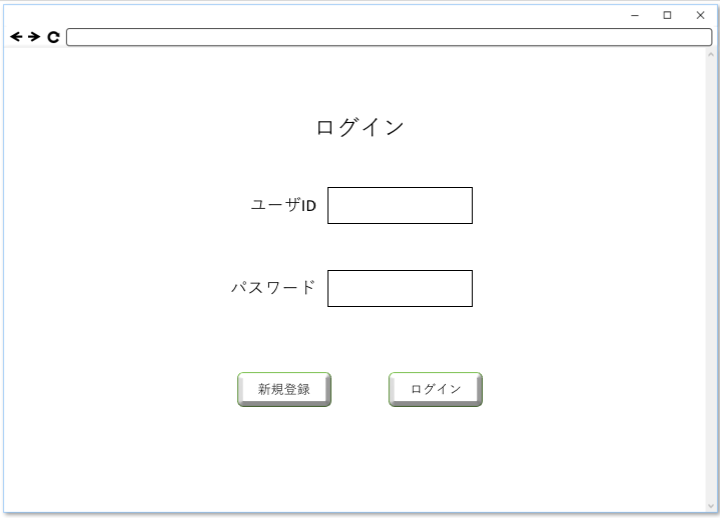
\includegraphics[width=1\linewidth,clip]{./img/01.png}
    \caption{ログイン画面のイメージ図}\label{fig:01}
  \end{center}
\end{figure}

\begin{figure}[phtbp]
  \begin{center}
    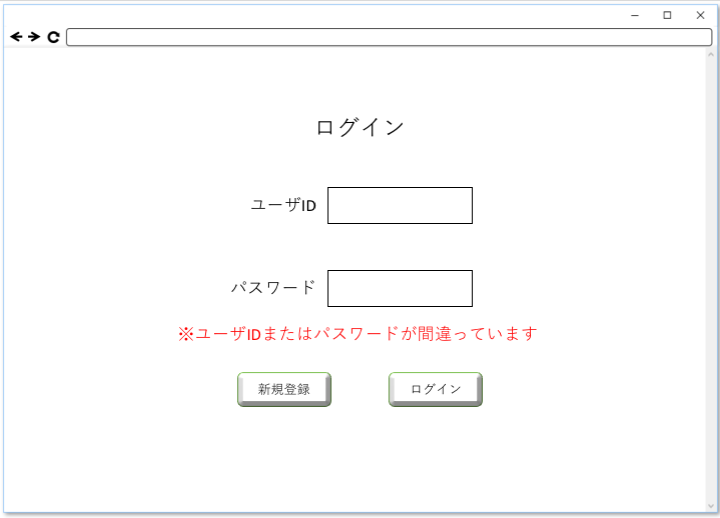
\includegraphics[width=1\linewidth,clip]{./img/02.png}
    \caption{ログイン画面のエラー表示イメージ図}\label{fig:02}
  \end{center}
\end{figure}

\newpage

\subsection{アカウント新規作成画面}
\subsubsection{画面の概要}
% 画面の概要
この画面は、学生がアカウントを新規作成するためのものです。
図\ref{fig:03}にイメージ図を示します。

\subsubsection{操作説明}
% 操作説明
ユーザID、氏名(フルネーム)およびパスワードを入力します。
なお、パスワードは確認のために2回入力します。
「登録」ボタンをクリックするとアカウントが登録され、「ログイン画面」に遷移します。

\begin{figure}[htbp]
  \begin{center}
    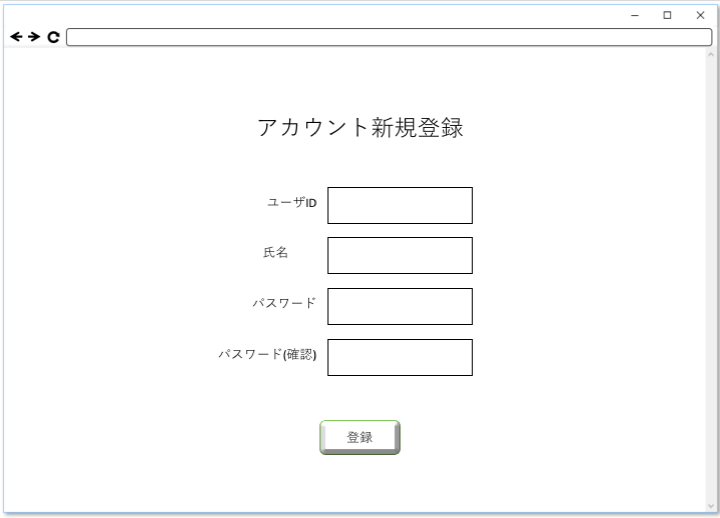
\includegraphics[width=1\linewidth,clip]{./img/03.png}
    \caption{アカウント新規作成画面のイメージ図}\label{fig:03}
  \end{center}
\end{figure}

\newpage

\subsection{管理者用ホーム画面}
\subsubsection{画面の概要}
% 画面の概要
この画面は、管理者がログインした際に表示されるものです。
図\ref{fig:04}にイメージ図を示します。

これ以降に表示される、この画面の右上にある「◯◯がログイン中」というのは、今誰がログインしているかを表しており、これの右にある逆三角をクリックすると、アカウントの登録情報を変更する画面への遷移やログアウトができるようになっています。
図\ref{fig:05}にイメージ図を示します。

\subsubsection{操作説明}
% 操作説明
右上にはログインしたユーザの氏名が表示されており、「登録情報編集」ボタンを押すことで「登録情報編集画面」に遷移します。また、「ログアウト」ボタンを押すことで、ログアウトし「ログイン画面」に遷移します。
「アカウント新規作成」ボタンを押すと、他のユーザのアカウント作成することができる、「他のアカウント新規登録画面」に遷移します。
「授業選択・作成」ボタンを押すと、「授業選択画面」に遷移します。また、画面左の最近開いた授業の欄には、最近編集または使用した授業が最大6つ分リンクが表示されています。

\begin{figure}[phtbp]
  \begin{center}
    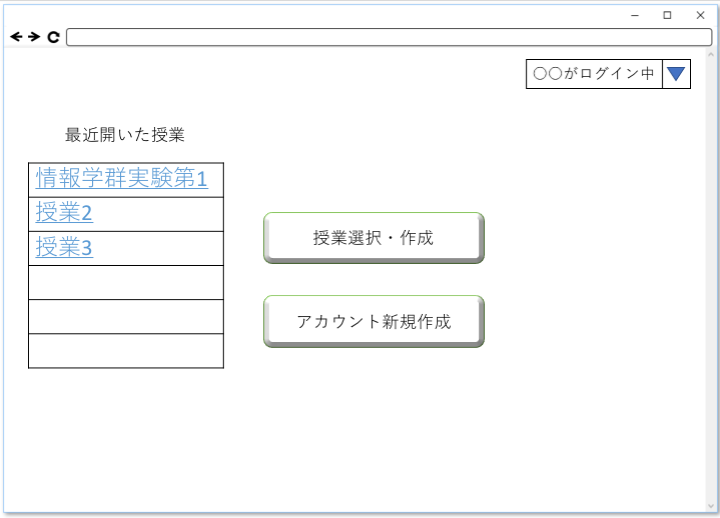
\includegraphics[width=1\linewidth,clip]{./img/04.png}
    \caption{管理者用ホーム画面のイメージ図}\label{fig:04}
  \end{center}
\end{figure}

\begin{figure}[phtbp]
  \begin{center}
    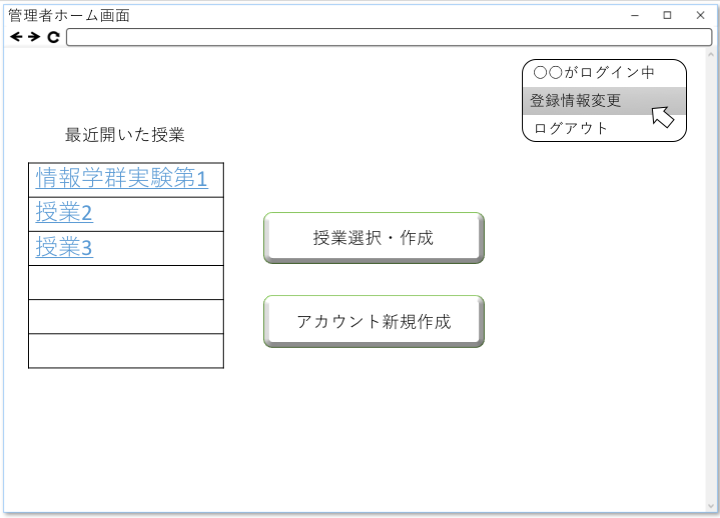
\includegraphics[width=1\linewidth,clip]{./img/05.png}
    \caption{画面右上選択のイメージ図}\label{fig:05}
  \end{center}
\end{figure}

\newpage

\subsection{登録情報編集画面}
\subsubsection{画面の概要}
% 画面の概要
この画面は、ユーザの登録したユーザIDやパスワードなどの登録情報を編集することができる画面です。
図\ref{fig:06}にイメージ図を示します。

\subsubsection{操作説明}
% 操作説明
旧パスワードの欄には現在使用しているパスワードを入力し、新パスワードの欄には新しく設定したいパスワードを入力します。ここでも確認のため、新パスワードをもう一度入力します。
ユーザ情報の編集が終われば、「変更」ボタンを押すことで、編集内容が保存されて「管理者ホーム画面」に遷移します。

\begin{figure}[htbp]
  \begin{center}
    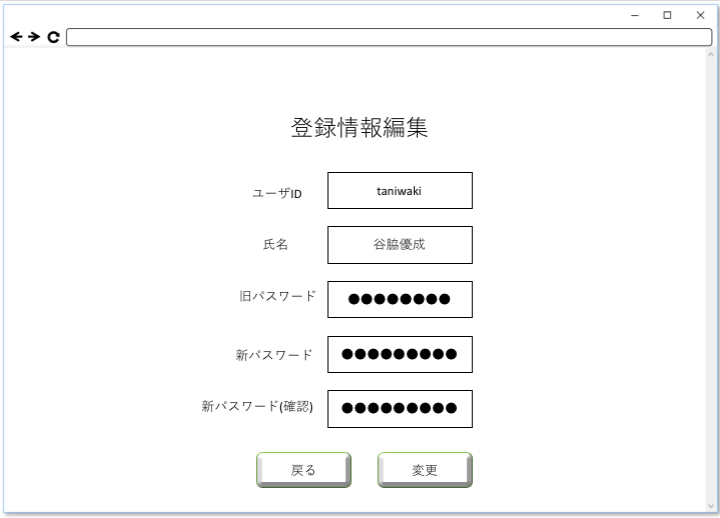
\includegraphics[width=1\linewidth,clip]{./img/06.png}
    \caption{登録情報編集画面のイメージ図}\label{fig:06}
  \end{center}
\end{figure}

\newpage

\subsection{他のアカウント新規登録画面}
\subsubsection{画面の概要}
% 画面の概要
この画面は、管理者側が自分以外のアカウントを新規登録する際の画面です。主に、新しく教員や授業のアシスタントを登録するときなどに使われます。

図\ref{fig:07}、\ref{fig:08}にイメージ図を示します。

\subsubsection{操作説明}
% 操作説明
権限レベルの逆三角を押すことで教員、アシスタント、学生の3つから権限レベルを指定することができ、登録するアカウントを区別します。
アカウント登録後、登録したアカウントを実際に使用する人にパスワードの変更を行ってもらうようにしてください。

\begin{figure}[phtbp]
  \begin{center}
    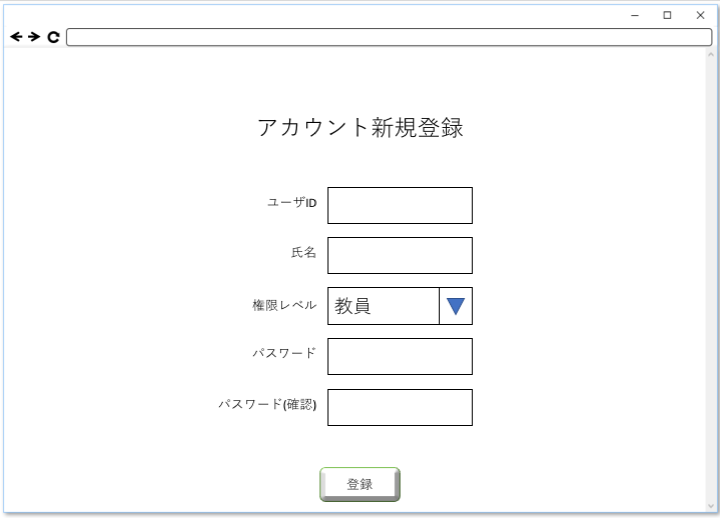
\includegraphics[width=1\linewidth,clip]{./img/07.png}
    \caption{管理者用の他のアカウント新規作成画面のイメージ図}\label{fig:07}
  \end{center}
\end{figure}

\begin{figure}[phtbp]
  \begin{center}
    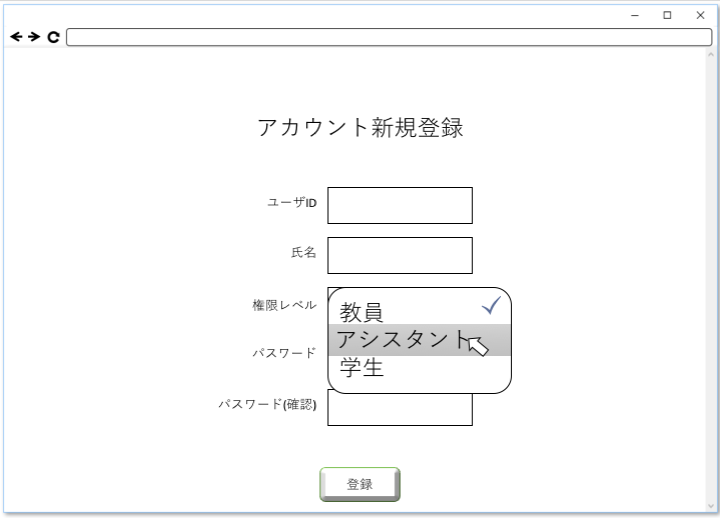
\includegraphics[width=1\linewidth,clip]{./img/08.png}
    \caption{権限レベル選択のイメージ図}\label{fig:08}
  \end{center}
\end{figure}

\newpage

\subsection{授業選択画面}
\subsubsection{画面の概要}
% 画面の概要
この画面は、授業の開講、質問の閲覧・編集、グループの編集などを行うときに対象となる授業を選択する画面です。また、この画面から、授業の新規作成を行う「授業新規作成画面」や、作成している授業に関する編集を行う「詳細設定画面2」に遷移できる画面でもあります。
図\ref{fig:09}にイメージ図を示します。

\subsubsection{操作説明}
% 操作説明
管理者が作成した授業のリンクが表示されており、そのリンクをクリックすることでその授業の「管理者用の授業回選択画面」に遷移します。
新しい授業を作成したい場合は、「授業新規作成」ボタンを押すことで、「授業新規作成画面」に遷移します。
また、すでに作成している授業の情報を編集したい場合、授業名の横の「編集」ボタンを押すことで、「詳細設定画面2」に遷移します。

\begin{figure}[htbp]
  \begin{center}
    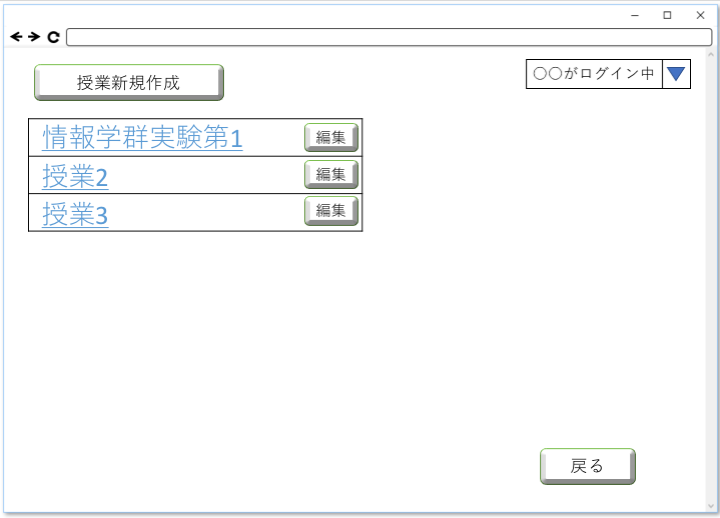
\includegraphics[width=1\linewidth,clip]{./img/09.png}
    \caption{授業選択画面のイメージ図}\label{fig:09}
  \end{center}
\end{figure}

\newpage

\subsection{授業新規作成画面}
\subsubsection{画面の概要}
% 画面の概要
この画面は、新しく授業を作成する時の、初期設定を行う画面です。
授業名、個人ワークかグループワーク、質問機能+進捗機能か質問機能のみ、の3つを決めることができます。
図\ref{fig:10}にイメージ図を示します。

\subsubsection{操作説明}
% 操作説明
まず、授業名を入力します。
その後、グループワークなのか、個人ワークなのかを選択し、最後に使用する機能が質問機能と進捗機能なのか、それとも質問機能だけなのかを選択し、「決定」ボタンを押すことで、「詳細設定画面」に遷移します。

\begin{figure}[htbp]
  \begin{center}
    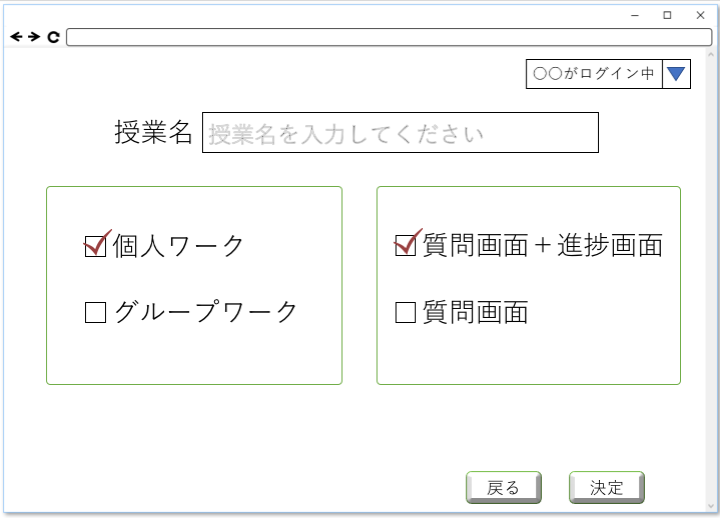
\includegraphics[width=1\linewidth,clip]{./img/10.png}
    \caption{授業新規作成画面のイメージ図}\label{fig:10}
  \end{center}
\end{figure}

\newpage

\subsection{詳細設定画面1}
\subsubsection{画面の概要}
% 画面の概要
この画面は、授業回ごとの授業タイトルや課題数を設定する画面です。
また、作成、編集している授業をグループワークで行う場合に、グループの編集が行える画面に遷移できる画面でもあります。
この遷移は「詳細設定画面2」や「詳細設定画面3」でも行えます。
図\ref{fig:11}にイメージ図を示します。

\subsubsection{操作説明}
% 操作説明
授業タイトルには学生側が過去の質問を見ようとした時でもわかるようなタイトルを入力し、課題数にはその回に出る課題の数を入力します。
授業回数を増やしたい場合は、「授業を追加する」ボタンを押すことで、その回の入力欄が追加されていきます。
全ての入力が終われば、「決定」ボタンを押すことで入力内容が保存され、「詳細設定画面2」に遷移します。
また、「グループ編集」ボタンを押すことで、「グループ編集選択画面」に遷移できます。

\begin{figure}[htbp]
  \begin{center}
    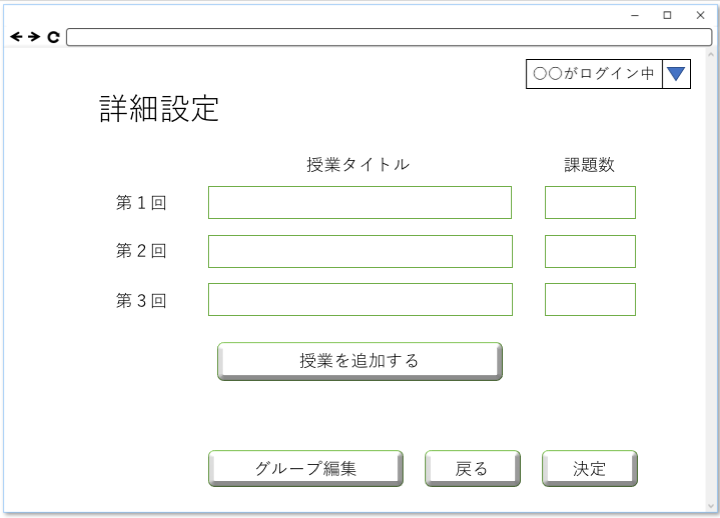
\includegraphics[width=1\linewidth,clip]{./img/11.png}
    \caption{詳細設定画面1のイメージ図}\label{fig:11}
  \end{center}
\end{figure}

\newpage

\subsection{詳細設定画面2}
\subsubsection{画面の概要}
% 画面の概要
この画面は「詳細設定画面1」で入力したタイトルとその課題数に応じて課題の内容を入力できる画面に遷移できる画面です。
図\ref{fig:12}にイメージ図を示します。

\subsubsection{操作説明}
% 操作説明
授業タイトルのボタンを押すことでその回の課題内容を入力する「詳細設定画面3」に遷移します。
「詳細設定画面3」に全ての回に応じた課題内容を入力し終わったら、「決定」ボタンを押すことで授業ページが作成されます。
授業タイトルや課題数を編集したり、授業回を新しく追加したい場合は、「授業の追加・編集」ボタンを押すことで「詳細設定画面1」に遷移できます。

\begin{figure}[htbp]
  \begin{center}
    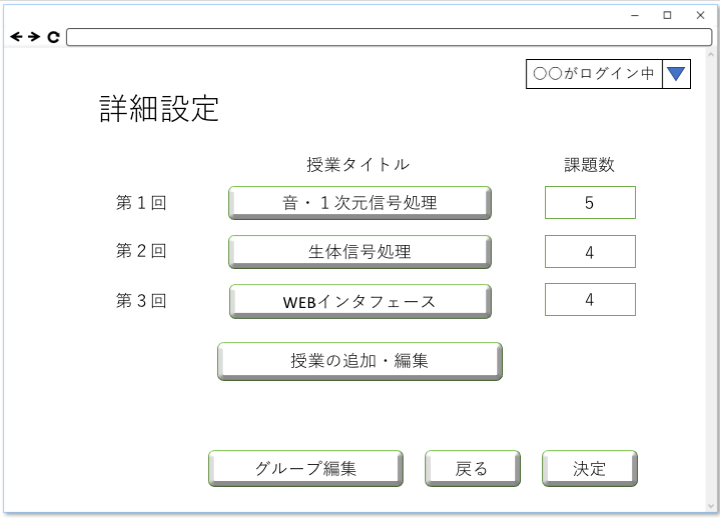
\includegraphics[width=1\linewidth,clip]{./img/12.png}
    \caption{詳細設定画面2のイメージ図}\label{fig:12}
  \end{center}
\end{figure}

\newpage

\subsection{詳細設定画面3}
\subsubsection{画面の概要}
% 画面の概要
この画面は、授業回ごとに課題の内容や、「進捗確認画面」で表示される課題名などを設定する画面です。
図\ref{fig:13}にイメージ図を示します。

\subsubsection{操作説明}
% 操作説明
画面左側に「詳細設定画面1」で入力した、課題数分の課題内容を入力するテキストボックスが表示されます。
そのテキストボックス内に課題の内容を入力することで課題内容を設定できます。
画面右側には、進捗確認画面や質問の確認などでカテゴリとして表示される課題名を入力できます。
「決定」ボタンを押すことで内容が確定され、「詳細設定画面2」に戻ります。

\begin{figure}[htbp]
  \begin{center}
    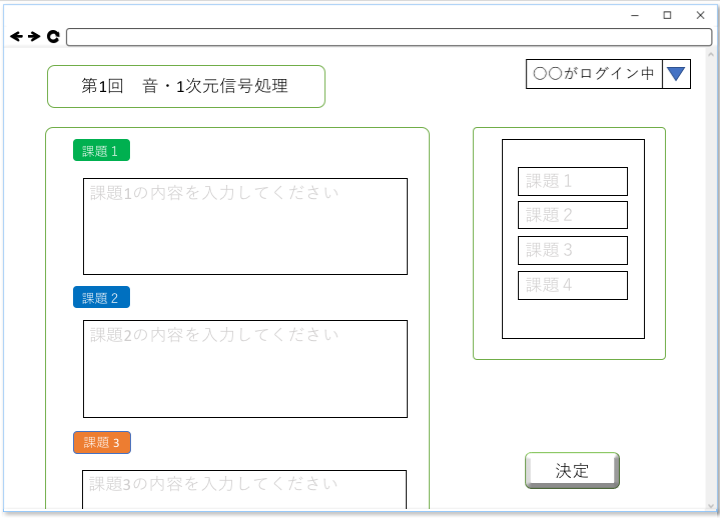
\includegraphics[width=1\linewidth,clip]{./img/13.png}
    \caption{詳細設定画面3のイメージ図}\label{fig:13}
  \end{center}
\end{figure}

\newpage

\subsection{編集グループ選択画面}
\subsubsection{画面の概要}
% 画面の概要
この画面は、管理者が編集したいグループを選択する画面です。
また、グループの新規作成を行うこともできます。
図\ref{fig:14}にイメージ図を示します。

\subsubsection{操作説明}
% 操作説明
グループ名のボタンを押すことで、グループの詳細ウィンドウが表示され、「編集」ボタンを押すことで、
そのグループの「グループ編集情報画面」に遷移します。
また、「新規グループ作成」ボタンを押すことで、グループを作成することができます。

\begin{figure}[htbp]
  \begin{center}
    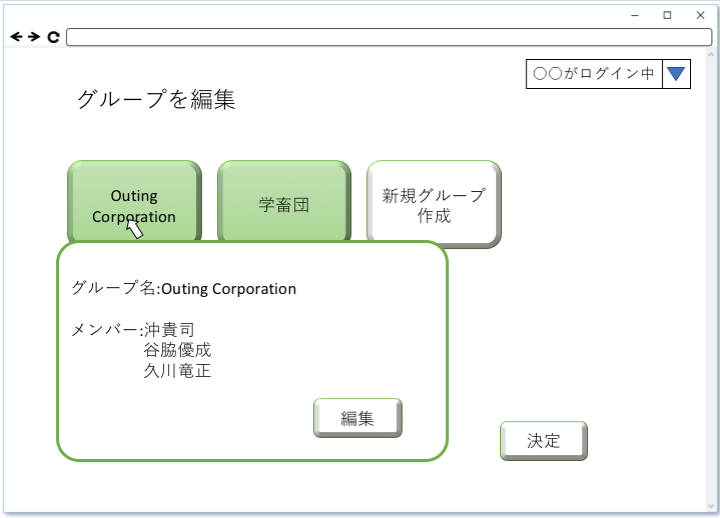
\includegraphics[width=1\linewidth,clip]{./img/14.png}
    \caption{編集グループ選択画面のイメージ図}\label{fig:14}
  \end{center}
\end{figure}

\newpage

\subsection{グループ情報編集画面}
\subsubsection{画面の概要}
% 画面の概要
この画面は、管理者が作成されているグループ名の編集および、グループやユーザの削除が行える画面です。
図\ref{fig:15}にイメージ図を示します。

\subsubsection{操作説明}
% 操作説明
グループ名が記載されている部分はテキストを直接編集することができます。
ユーザやグループ自体を削除する場合は、削除対象の右にあるチェックボックスにチェックを入れて、「削除」ボタンを押すことで削除を行うことができます。
最後に「決定」ボタンを押すことで、編集内容を保存し「編集グループ選択画面」に遷移します。

\begin{figure}[htbp]
  \begin{center}
    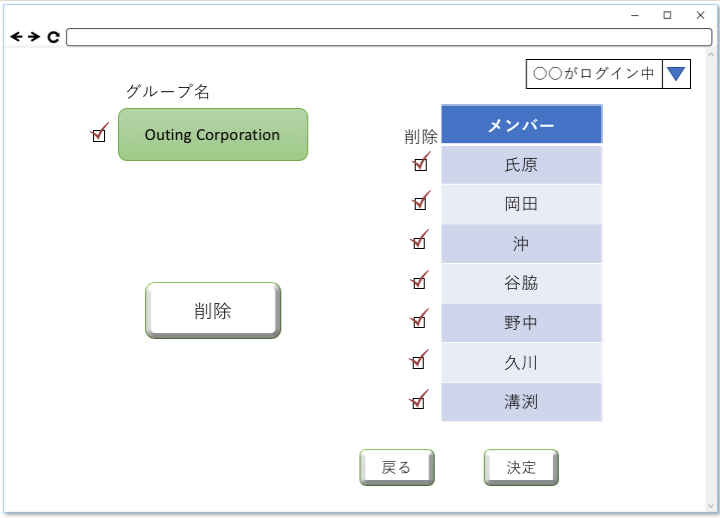
\includegraphics[width=1\linewidth,clip]{./img/15.png}
    \caption{グループ情報編集画面のイメージ図}\label{fig:15}
  \end{center}
\end{figure}

\newpage

\subsection{管理者用の授業回選択画面}
\subsubsection{画面の概要}
% 画面の概要
この画面は、使用したい授業の回を選択する画面です。
図\ref{fig:16}にイメージ図を示します。

\subsubsection{操作説明}
% 操作説明
授業タイトルのボタンを押すことで、その回の授業の「進捗確認画面」に遷移します。
「質問閲覧・編集」ボタンを押すことで、「質問閲覧・編集画面1」に遷移します。

\begin{figure}[htbp]
  \begin{center}
    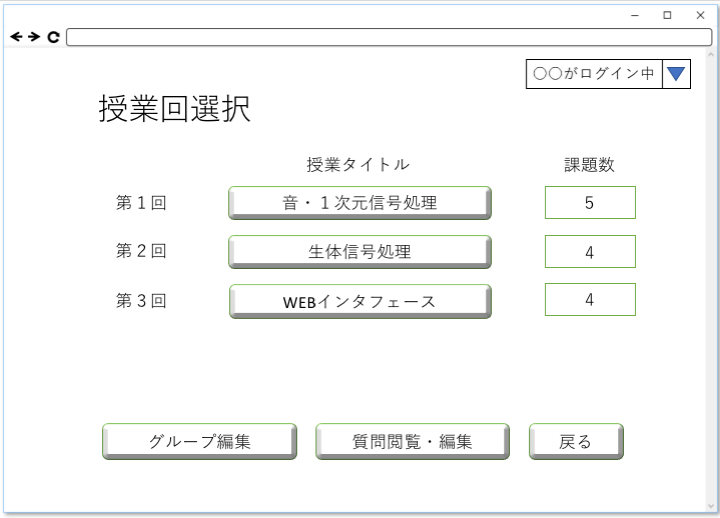
\includegraphics[width=1\linewidth,clip]{./img/16.png}
    \caption{管理者用の授業回選択画面のイメージ図}\label{fig:16}
  \end{center}
\end{figure}

\newpage

\subsection{質問閲覧・編集画面1}
\subsubsection{画面の概要}
% 画面の概要
この画面は、質問閲覧・編集を行いたい授業が行われた年度を選択する画面です。
図\ref{fig:17}にイメージ図を示します。

\subsubsection{操作説明}
% 操作説明
年度の書かれたボタンを押すことで、その年度に開かれた授業が回ごとに並んでいる「質問閲覧・編集画面2」に遷移します。

\begin{figure}[htbp]
  \begin{center}
    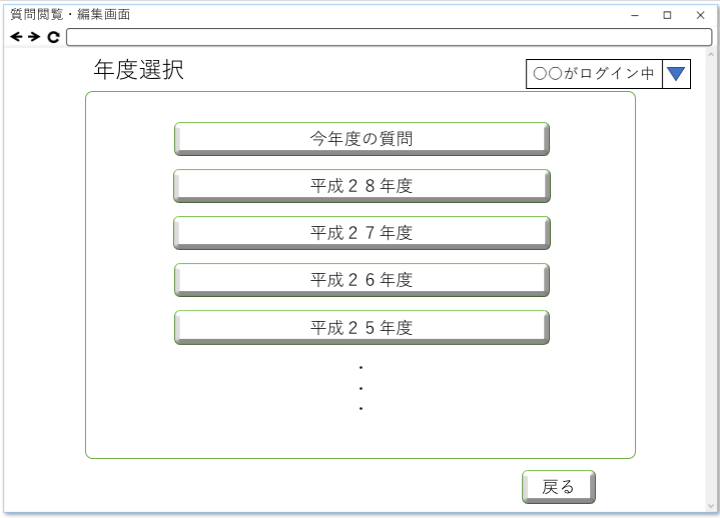
\includegraphics[width=1\linewidth,clip]{./img/17.png}
    \caption{質問閲覧・編集画面1のイメージ図}\label{fig:17}
  \end{center}
\end{figure}

\newpage

\subsection{質問閲覧・編集画面2}
\subsubsection{画面の概要}
% 画面の概要
この画面は、質問の閲覧・編集を行いたい授業回を選択する画面です。
図\ref{fig:18}にイメージ図を示します。

\subsubsection{操作説明}
% 操作説明
質問の閲覧や編集を行いたい授業回が書かれているボタンをクリックすることで、
その授業回の「質問閲覧・編集画面3」に遷移します。

\begin{figure}[htbp]
  \begin{center}
    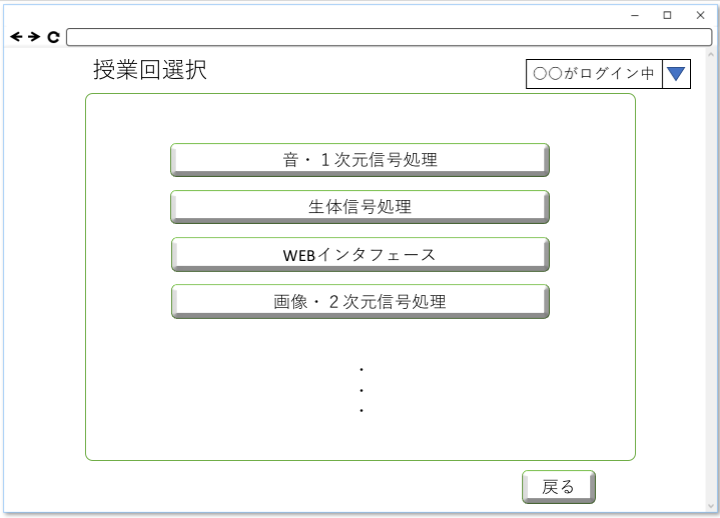
\includegraphics[width=1\linewidth,clip]{./img/18.png}
    \caption{質問閲覧・編集画面2のイメージ図}\label{fig:18}
  \end{center}
\end{figure}

\newpage

\subsection{質問閲覧・編集画面3}
\subsubsection{画面の概要}
% 画面の概要
この画面は、データベースに蓄積されている質問を閲覧・編集できる画面です。
図\ref{fig:19}、\ref{fig:000}にイメージ図を示します。

\subsubsection{操作説明}
% 操作説明
質問内容や回答を直接クリックすると編集することができるようになります。
また、非公開のチェックボックスによって学生へその質問を公開するかどうかを選択することができます。
「削除」ボタンでは、その質問自体を削除することができます。

\begin{figure}[htbp]
  \begin{center}
    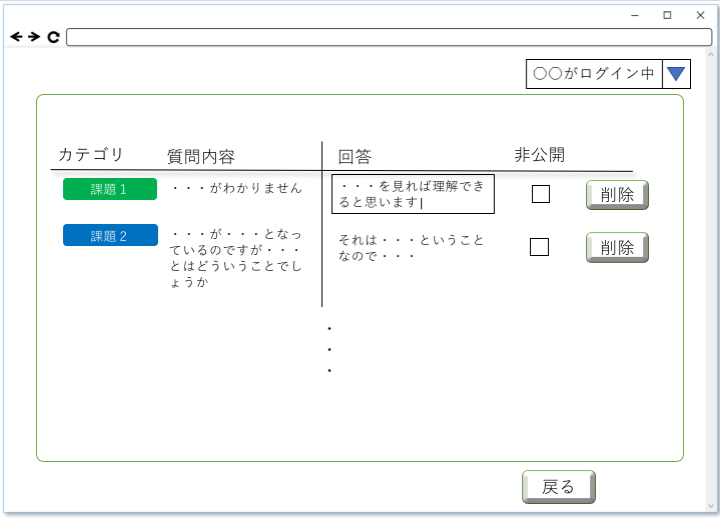
\includegraphics[width=1\linewidth,clip]{./img/19.png}
    \caption{質問閲覧・編集画面3のイメージ図}\label{fig:19}
  \end{center}
\end{figure}

\begin{figure}[htbp]
  \begin{center}
    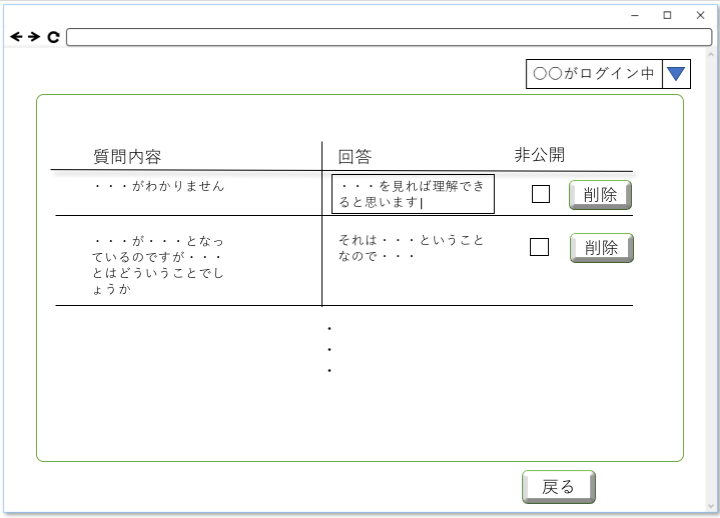
\includegraphics[width=1\linewidth,clip]{./img/000.png}
    \caption{質問閲覧・編集画面3のイメージ図(質問機能のみ)}\label{fig:000}
  \end{center}
\end{figure}

\newpage

\subsection{進捗確認画面}
\subsubsection{画面の概要}
% 画面の概要
この画面は、授業時に使用される学生の課題の進捗状況を確認する画面です。
図\ref{fig:20}、図\ref{fig:21}にグループでのイメージ図を示します。
図\ref{fig:22}、図\ref{fig:23}に個人でのイメージ図を示します。

\subsubsection{操作説明}
% 操作説明
表の形式でユーザごとの進捗が表示されており、氏名の横に課題ごとの進捗が表示されます。%氏名の横かな〜
また、学生から質問があると、その学生の一番右側の状態の欄に黄色のアイコンが表示され、
課題の確認の場合は緑色のアイコン、緊急の場合は赤色のアイコンが表示されます。
画面右下の「課題編集」ボタンを押すことで、今開講している授業の課題内容の編集が行える、「詳細設定画面3」に遷移します。
表内を押すと、その押した行にあるユーザからの質問確認が行えるウィンドウが開き、そのウィンドウの「回答」ボタンを押すことで、%行の
「質問回答画面」に遷移します。


\begin{figure}[phtbp]
  \begin{center}
    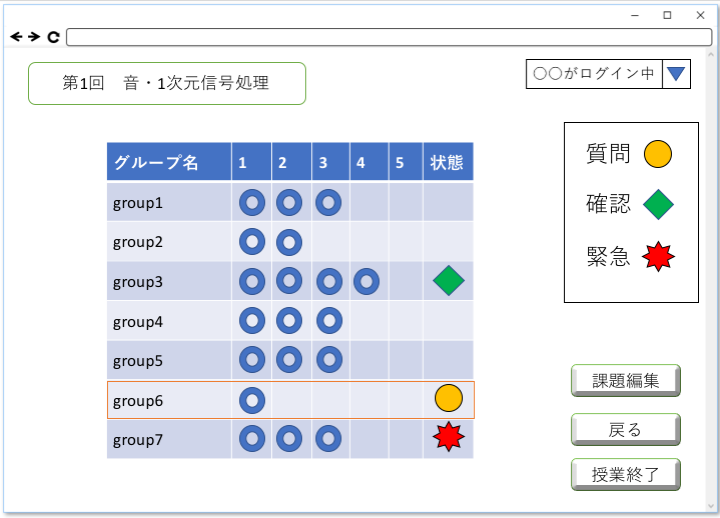
\includegraphics[width=1\linewidth,clip]{./img/20.png}
    \caption{進捗確認画面のイメージ図(グループ)}\label{fig:20}
  \end{center}
\end{figure}

\begin{figure}[phtbp]
  \begin{center}
    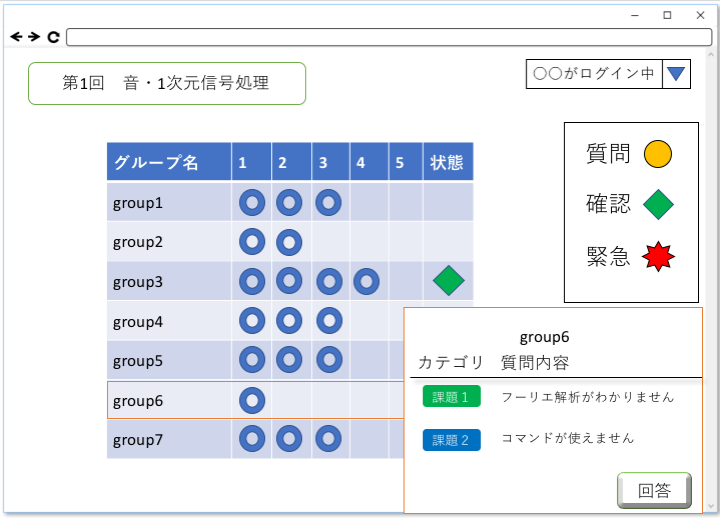
\includegraphics[width=1\linewidth,clip]{./img/21.png}
    \caption{進捗確認画面のイメージ図2(グループ)}\label{fig:21}
  \end{center}
\end{figure}

\begin{figure}[phtbp]
  \begin{center}
    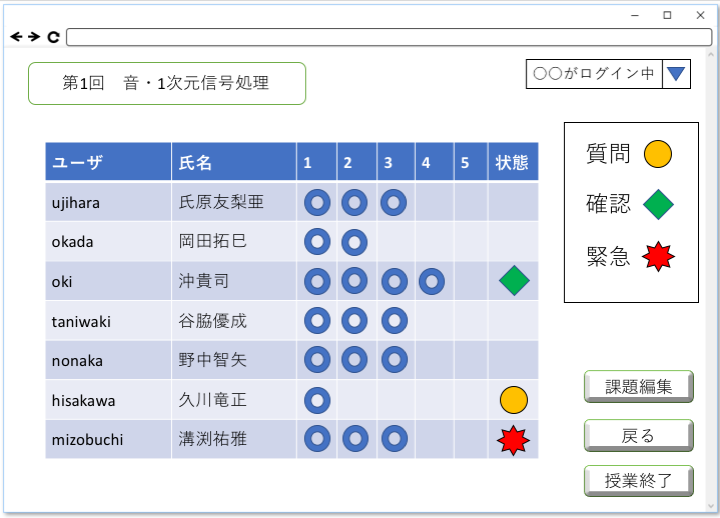
\includegraphics[width=1\linewidth,clip]{./img/22.png}
    \caption{進捗確認画面のイメージ図(個人)}\label{fig:22}
  \end{center}
\end{figure}

\begin{figure}[phtbp]
  \begin{center}
    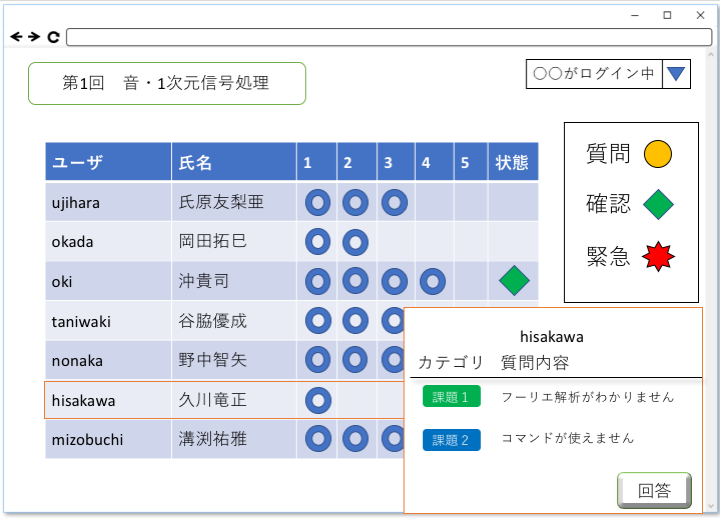
\includegraphics[width=1\linewidth,clip]{./img/23.png}
    \caption{進捗確認画面のイメージ図2(個人)}\label{fig:23}
  \end{center}
\end{figure}

\newpage

\subsection{質問回答画面}
\subsubsection{画面の概要}
% 画面の概要
この画面には、左側にグループ名と、そのグループからの質問が表示されています。
図\ref{fig:24}、\ref{fig:25}にイメージ図を示します。

\subsubsection{操作説明}
% 操作説明
質問へ回答をしたい場合、その質問が表示されている部分を選択した後、右側にある回答記入欄に回答を記入し、「回答」ボタンをクリックすることで送信します。
質問や回答の内容は他の学生も閲覧することが可能となっており、その質問や回答の内容を公開するかどうかは、質問の横にある非公開のチェックボックスによって設定ができます。

\begin{figure}[phtbp]
  \begin{center}
    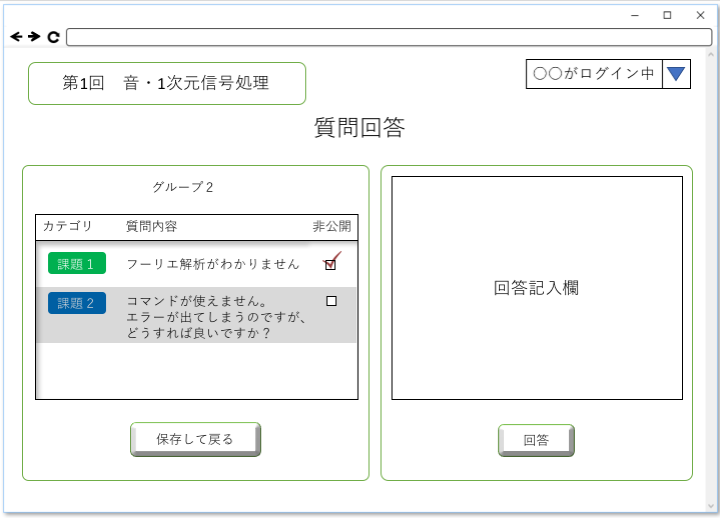
\includegraphics[width=1\linewidth,clip]{./img/24.png}
    \caption{質問回答画面(課題に対する質問)}\label{fig:24}
  \end{center}
\end{figure}

\begin{figure}[phtbp]
  \begin{center}
    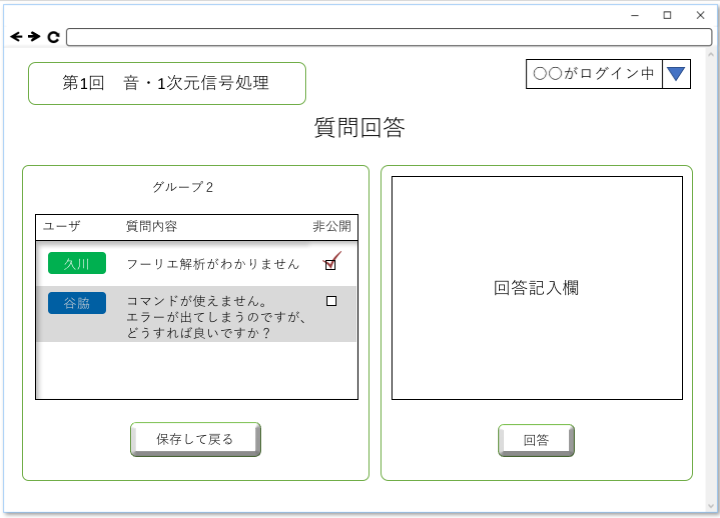
\includegraphics[width=1\linewidth,clip]{./img/25.png}
    \caption{質問回答画面(授業に対する質問)}\label{fig:25}
  \end{center}
\end{figure}

\newpage

\subsection{グループ参加・作成画面}
\subsubsection{画面の概要}
% 画面の概要
この画面は、開講されている授業がグループで行う授業であり、まだどのグループにも参加していない場合に、ログインすると表示される画面です。
この画面では、すでに作成されているグループへの参加と、新規グループの作成が行えます。
図\ref{fig:26}、\ref{fig:27}にイメージ図を示します。

\subsubsection{操作説明}
% 操作説明

作成されているグループに参加する場合、参加したいグループ名の書かれたボタンを押します。
するとウィンドウが表示され、中にグループ名と現状参加しているメンバーが表示されるので、
内容を確認して参加する場合、「参加」ボタンを押してグループへの参加を完了します。
グループを間違えた場合は、ウィンドウ外をクリックして画面を閉じます。

グループを作成する場合、「新規グループ作成」ボタンを押します。
ウィンドウが表示されるので、グループ名を記入し、「作成」ボタンを押して作成を完了します。

\begin{figure}[phtbp]
  \begin{center}
    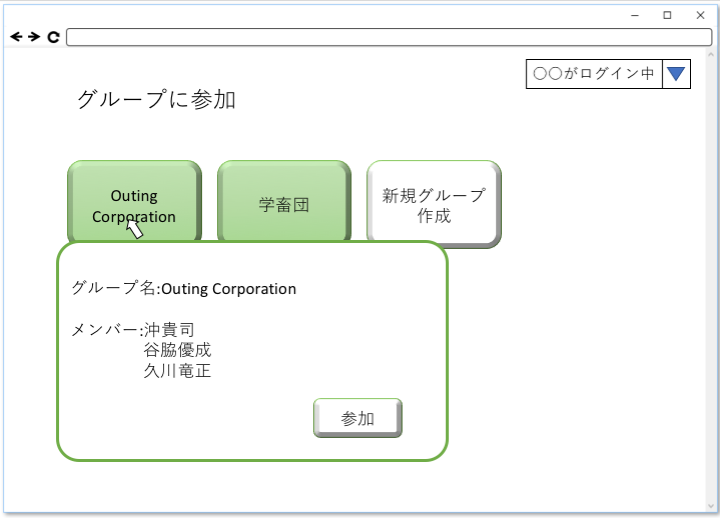
\includegraphics[width=1\linewidth,clip]{./img/26.png}
    \caption{グループ参加・作成画面のグループ参加イメージ図}\label{fig:26}
  \end{center}
\end{figure}

\begin{figure}[phtbp]
  \begin{center}
    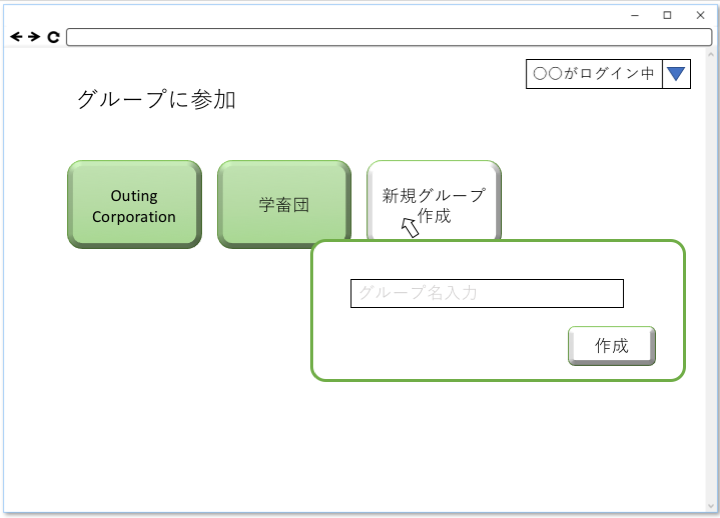
\includegraphics[width=1\linewidth,clip]{./img/27.png}
    \caption{グループ参加・作成画面のグループ作成イメージ図}\label{fig:27}
  \end{center}
\end{figure}

\newpage

\subsection{学生用のホーム画面}
\subsubsection{画面の概要}
% 画面の概要
この画面は、学生側のホーム画面です。
この画面では、今年度の質問を確認したり、進捗状況を管理者側に送信したりできます。
画面上部に授業名が表示されており、その下に質問確認欄と進捗状況入力欄があります。
左側の質問確認欄には、受講中の内容に関する質問が表示されており、カテゴリ順に並べられています。
ログイン時に授業が開講されていない場合はエラーが表示されます。
図\ref{fig:28}、\ref{fig:29}、\ref{fig:00}にイメージ図を示します。

\subsubsection{操作説明}
% 操作説明
過去の質問を確認する場合、質問確認欄にある「過去の質問」ボタンを押して「学生用の年度選択画面」に遷移します。
質問をする場合、質問確認欄にある「質問をする」ボタンを押して「質問入力画面」に遷移します。
進捗状況を管理者側に送信する場合、進捗状況入力欄にあるチェックボックスに終わった課題分チェックをつけて「更新」ボタンを押して更新を行います。
全ての課題を終えて管理者側に確認を行ってもらいたい場合、「確認」ボタンを押します。

\begin{figure}[phtbp]
  \begin{center}
    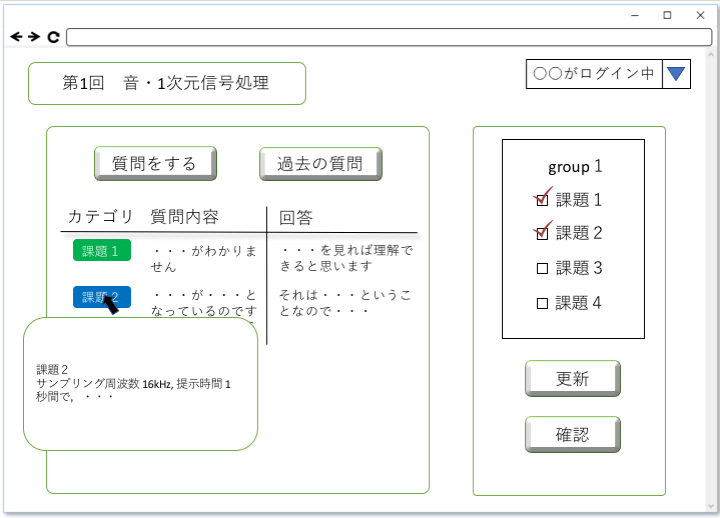
\includegraphics[width=1\linewidth,clip]{./img/28.png}
    \caption{学生用のホーム画面のイメージ図}\label{fig:28}
  \end{center}
\end{figure}

\begin{figure}[phtbp]
  \begin{center}
    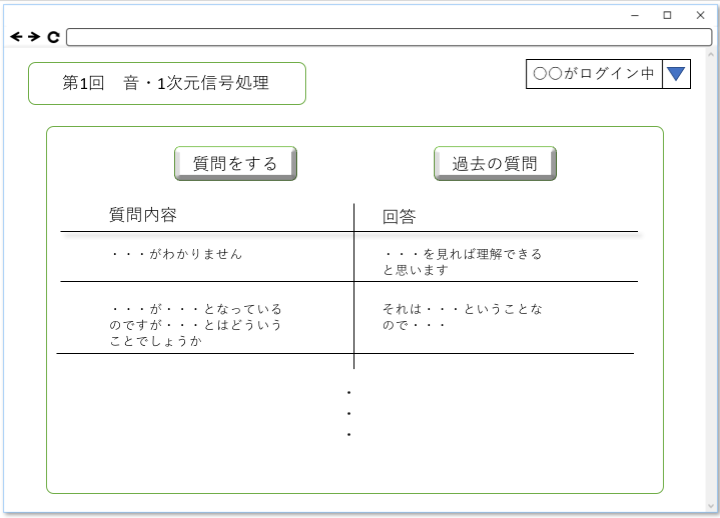
\includegraphics[width=1\linewidth,clip]{./img/29.png}
    \caption{学生用のホーム画面のイメージ図(質問機能のみ)}\label{fig:29}
  \end{center}
\end{figure}

\begin{figure}[phtbp]
  \begin{center}
    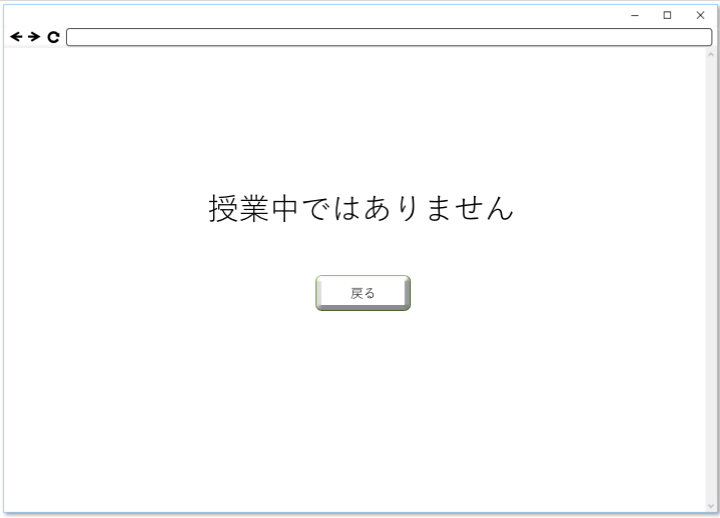
\includegraphics[width=1\linewidth,clip]{./img/00.png}
    \caption{学生用のホーム画面のエラー表示イメージ図}\label{fig:00}
  \end{center}
\end{figure}

\newpage

\subsection{学生用の年度選択画面}
\subsubsection{画面の概要}
% 画面の概要
この画面は、学生側が過去の質問を確認する際に、どの年度に出た質問を確認するのか選択する画面です。
図\ref{fig:30}、\ref{fig:31}にイメージ図を示します。

\subsubsection{操作説明}
% 操作説明
年度のボタンを押すと、その年度の「授業回選択画面」に遷移します。
「今年度の質問」ボタンを押すと今年度の質問が表示されている「学生用ホーム画面」に戻ります。

\begin{figure}[phtbp]
  \begin{center}
    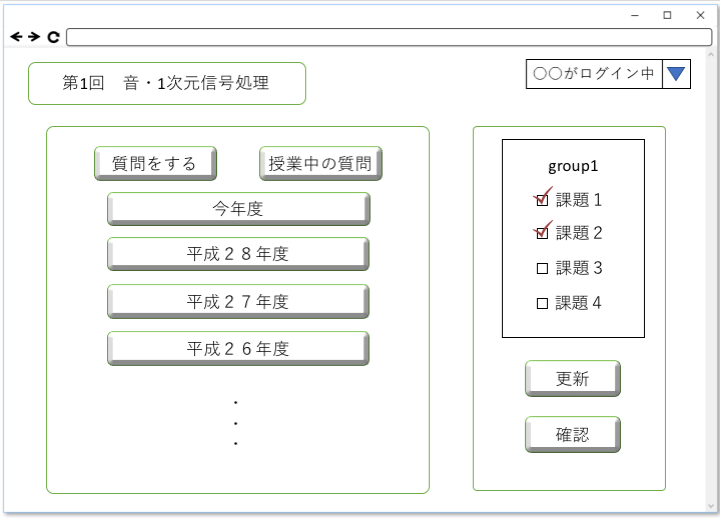
\includegraphics[width=1\linewidth,clip]{./img/30.png}
    \caption{学生用の年度選択画面のイメージ図}\label{fig:30}
  \end{center}
\end{figure}

\begin{figure}[phtbp]
  \begin{center}
    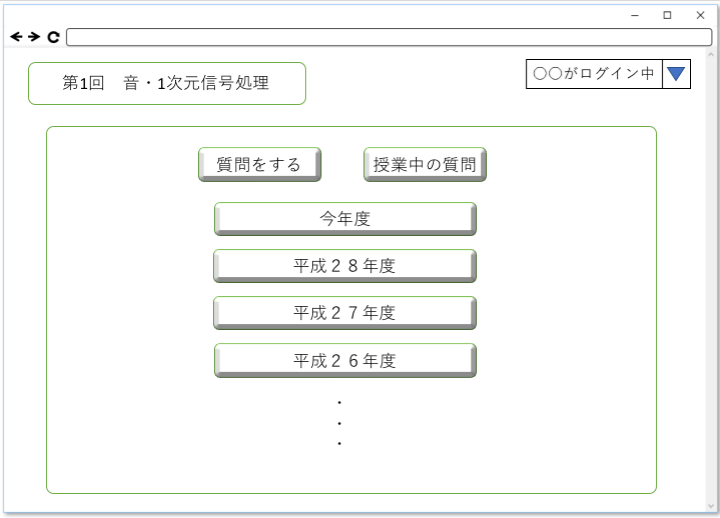
\includegraphics[width=1\linewidth,clip]{./img/31.png}
    \caption{学生用の年度選択画面のイメージ図(質問機能のみ)}\label{fig:31}
  \end{center}
\end{figure}

\newpage

\subsection{学生用の授業回選択画面}
\subsubsection{画面の概要}
% 画面の概要
この画面は、学生側が選択した質問を確認したい年度に対して、どの授業回か選択する画面です。
図\ref{fig:32}、\ref{fig:33}にイメージ図を示します。

\subsubsection{操作説明}
% 操作説明
授業回を選択するとその回の授業で出た質問が表示される「過去質問画面」に遷移します。
「年度選択」ボタンを押すと「年度選択画面」に戻ります。

\begin{figure}[phtbp]
  \begin{center}
    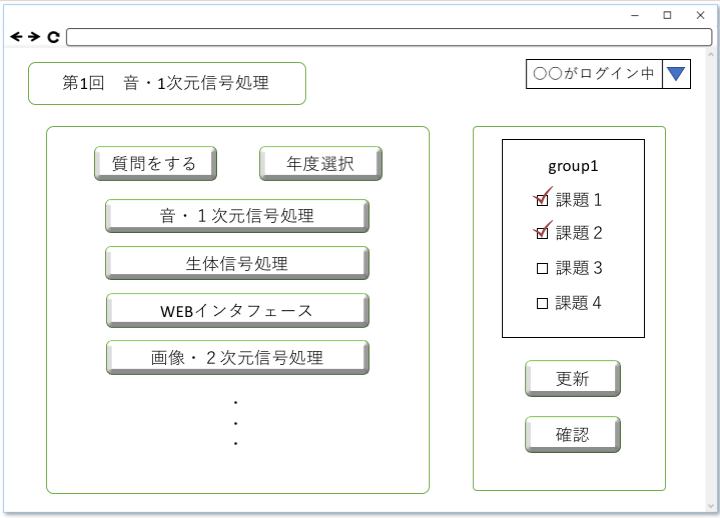
\includegraphics[width=1\linewidth,clip]{./img/32.png}
    \caption{学生用の授業回選択画面のイメージ図}\label{fig:32}
  \end{center}
\end{figure}

\begin{figure}[phtbp]
  \begin{center}
    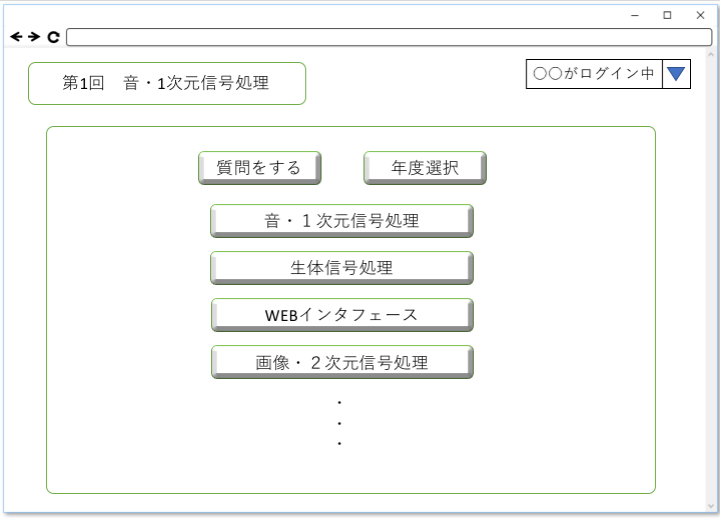
\includegraphics[width=1\linewidth,clip]{./img/33.png}
    \caption{学生用の授業回選択画面のイメージ図(質問機能のみ)}\label{fig:33}
  \end{center}
\end{figure}

\newpage

\subsection{学生用の過去質問画面}
\subsubsection{画面の概要}
% 画面の概要
この画面は、学生側が選択した条件に合わせて過去の質問が表示される画面です。
基本的に「学生用のホーム画面」と表示されていることは変わりませんが、「授業回選択」ボタンを押すことで
「授業回選択画面」に遷移します。
図\ref{fig:34}、\ref{fig:35}にイメージ図を示します。

\subsubsection{操作説明}
% 操作説明
「質問をする」ボタンを押すと他の画面同様、「質問入力画面」に移動します。
「授業回選択」ボタンを押すと、「学生用の授業回選択画面」へ戻ります。
2つのボタンの下には、選択した授業回について過去に出た質問が表示されます。

\begin{figure}[phtbp]
  \begin{center}
    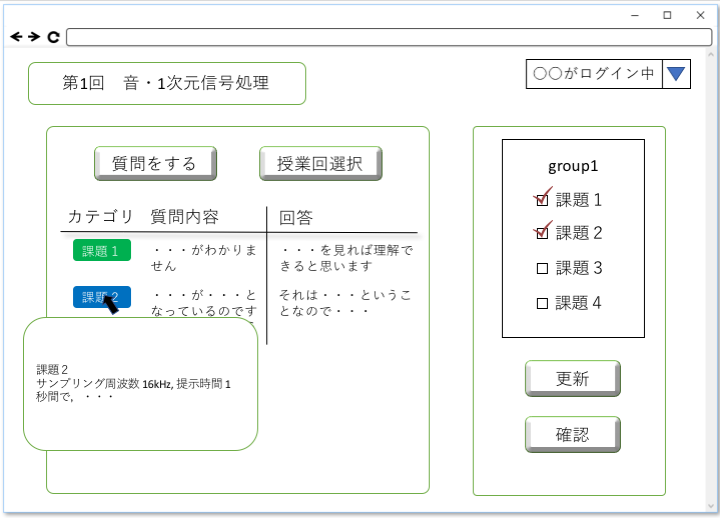
\includegraphics[width=1\linewidth,clip]{./img/34.png}
    \caption{学生用の過去質問画面のイメージ図}\label{fig:34}
  \end{center}
\end{figure}

\begin{figure}[phtbp]
  \begin{center}
    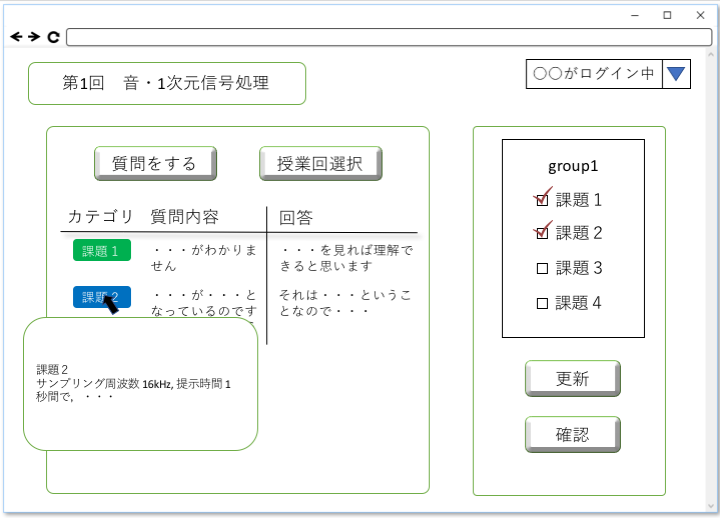
\includegraphics[width=1\linewidth,clip]{./img/35.png}
    \caption{学生用の過去質問画面のイメージ図(質問機能のみ)}\label{fig:35}
  \end{center}
\end{figure}

\newpage



\subsection{質問入力画面}
\subsubsection{画面の概要}
% 画面の概要
この画面は、学生側が管理者側に送信する質問内容を入力する画面です。
図\ref{fig:36}、\ref{fig:37}にイメージ図を示します。

\subsubsection{操作説明}
% 操作説明
まず画面上部の三角を押して、どの課題に対して質問をするのか選びます。
次にその下の質問入力欄に質問内容を入力して、「質問」ボタンを押します。
PCに問題が起きた時などの緊急案件の場合は課題選択のところに用意してあるその他を選んでいただき、
内容を書いて「緊急」ボタンを押していただきます。
2つのどのボタンを押しても管理者に内容を送信後、1つ手前の画面に戻ります。
課題がない授業の場合は、質問記入欄のみが画面に表示されます。
\begin{figure}[phtbp]
  \begin{center}
    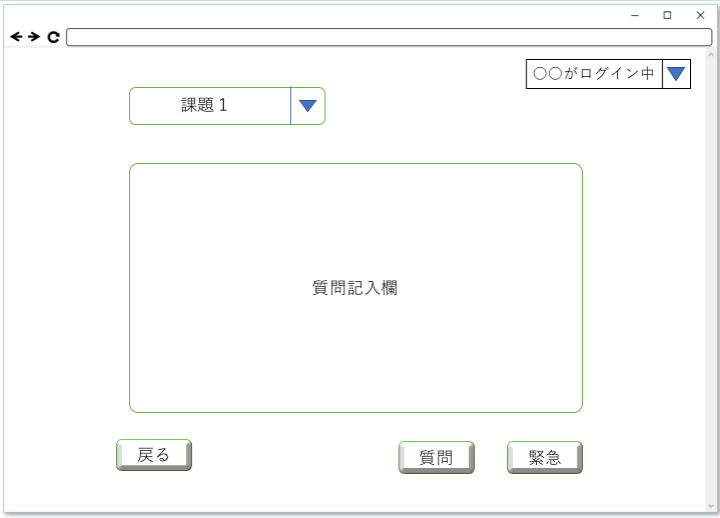
\includegraphics[width=1\linewidth,clip]{./img/36.png}
    \caption{質問入力画面のイメージ図}\label{fig:36}
  \end{center}
\end{figure}

\begin{figure}[phtbp]
  \begin{center}
    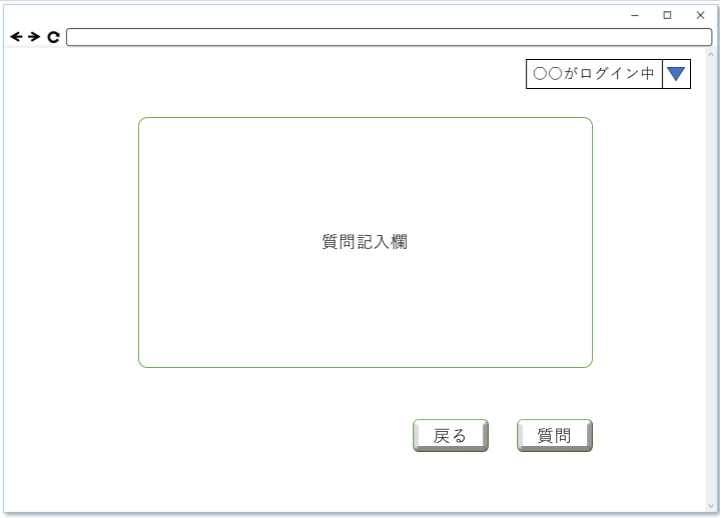
\includegraphics[width=1\linewidth,clip]{./img/37.png}
    \caption{質問入力画面のイメージ図(質問機能のみ)}\label{fig:37}
  \end{center}
\end{figure}

\newpage
